\documentclass[11pt,a4paper]{article}
\usepackage{fullpage}
\usepackage{graphicx}
\usepackage{float}

\newcommand*{\addheight}[2][.5ex]{%
  \raisebox{0pt}[\dimexpr\height+(#1)\relax]{#2}%
}

\title{\textbf{Chaotic Dynamics - CSCI 5446} \\
Problem Set 2}
\author{Santhanakrishnan Ramani}
\begin{document}
\maketitle
\section*{Problem 1}
\begin{figure}[H]
{
The Figure \ref{fig:prob1} represents the $m$ iterates of the logistic equation on the axes $x_{n}$ Vs $R$.\\ Value of $m = 600$, $l=300$, $2.8<R<4$, and the interval between R value is $0.01$ \par\bigskip
\centering 
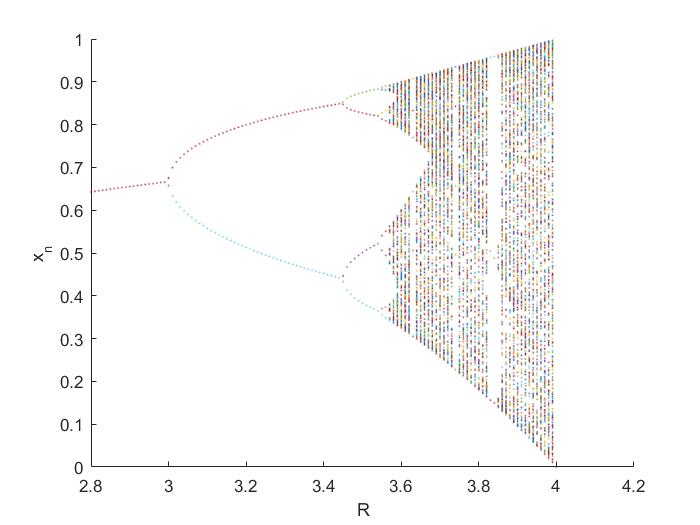
\includegraphics[scale=0.5]{images/prob1.jpg}
\caption{Bifurcation Plot}\par\medskip
\label{fig:prob1}
}
\end{figure}
\newpage
\section*{Problem 2}
\paragraph{•}
The Below Figure shows the places where bifurcation takes place for period 2,4,8,16.\\ \\
\begin{table}[H]
\centering
\begin{tabular}{|c|c|}
	\hline
	\addheight{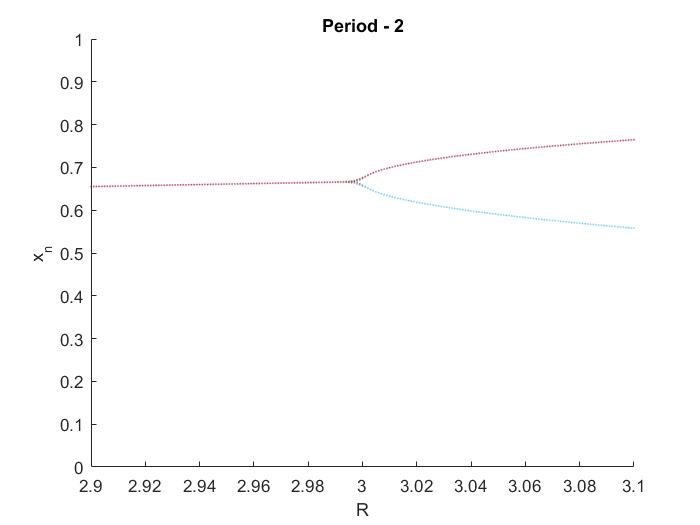
\includegraphics[width=80mm]{images/prob21.jpg}} &
    \addheight{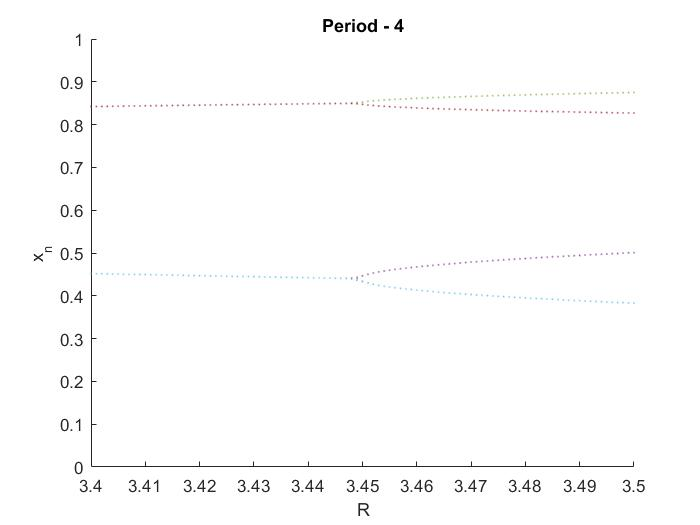
\includegraphics[width=80mm]{images/prob22.jpg}} \\
    \hline
    \addheight{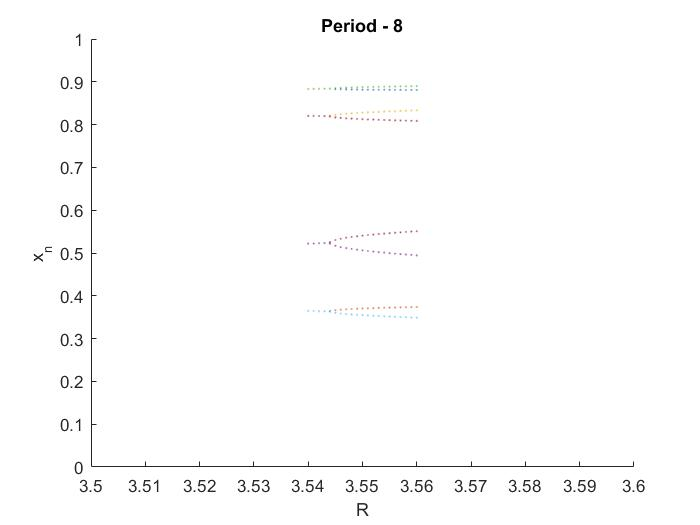
\includegraphics[width=80mm]{images/prob23.jpg}} &
    \addheight{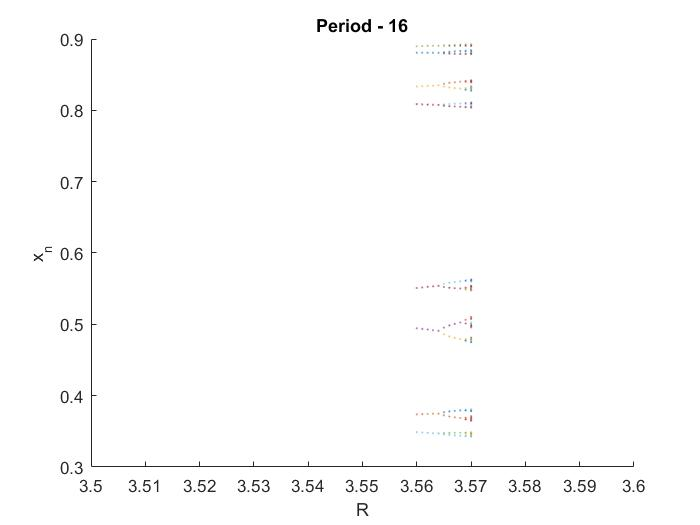
\includegraphics[width=80mm]{images/prob24.jpg}} \\
	\hline
\end{tabular}
\end{table}
\begin{table}[H]
\caption{Value of R where bifurcation takes place}
\centering\par\medskip
\begin{tabular}{|c|c|c|}
\hline
n & R & Period\\
\hline
1 & 3 & 2\\
2 & 3.449 & 4\\
3 & 3.544 & 8\\
4 & 3.564 & 16\\
\hline 
\end{tabular}
\end{table}

$$Feigenbaum\, number = \frac{r_{n} - r_{n-1}}{r_{n+1} - r_{n}}$$
\\
The Feigenbaum value obtained by substituting $n = 2 \,\&\, 3$ is $4.726 \,\&\, 4.657$ respectively. 
\section*{Problem 3}
\begin{figure}[H]
{
The Figure \ref{fig:prob3} and \ref{fig:prob31} represents the bifurcation plot of Henon Map with value of $m = 600$, $l=300$, $0<a<1.4$, $b=0.3$, and the interval between $a$ value is $0.01$ \par\bigskip
\centering 
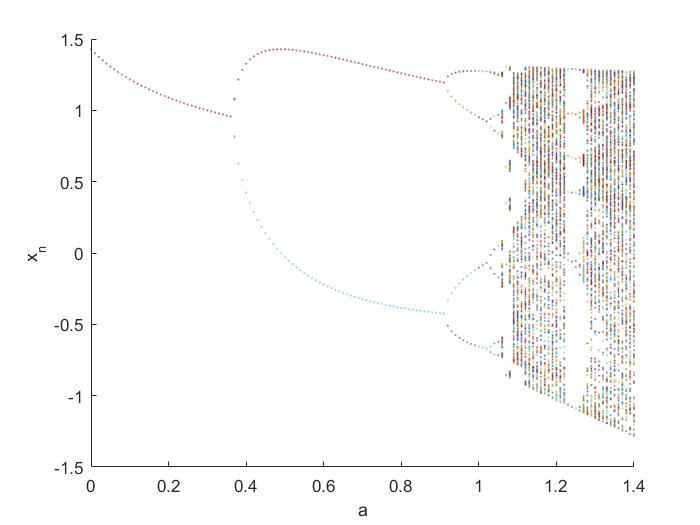
\includegraphics[scale=0.3]{images/prob3.jpg}
\caption{Bifurcation Plot}
\label{fig:prob3}
}
\end{figure}
\begin{figure}[H]
{
\centering 
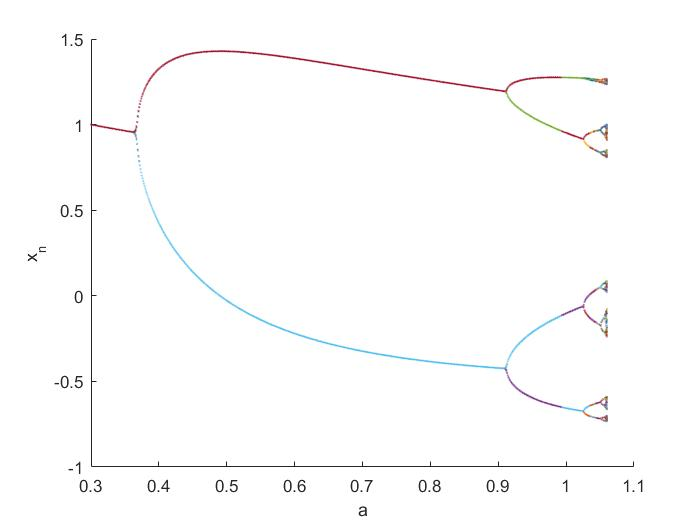
\includegraphics[scale=0.3]{images/prob31.jpg}
\caption{Bifurcation Plot}
\label{fig:prob31}
}
\end{figure}
\begin{table}[H]
\caption{Value of a where bifurcation takes place}
\centering\par\medskip
\begin{tabular}{|c|c|c|}
\hline
n & a & Period\\
\hline
1 & 0.364 & 2\\
2 & 0.912 & 4\\
3 & 1.026 & 8\\
4 & 1.051 & 16\\
\hline 
\end{tabular}
\end{table}
$$Feigenbaum\, number = \frac{a_{n} - a_{n-1}}{a_{n+1} - a_{n}}$$
\\
The Feigenbaum value obtained by substituting $n = 2 \,\&\, 3$ is $4.807 \,\&\, 4.715$ respectively.
\section*{Problem 4}
\begin{itemize}
	\item Yes, the answers of Problem 2 \,\&\, 3 are close and will be same as ${n\to\infty}$
	\item Yes, they should be the same as both the maps belongs to one parameter family of unimodal maps.
\end{itemize}
\end{document}
